
\labday{Jeudi, 21 avril 2016}
\label{day:21-04-2016}

Je vais résumer ici l'avancement du projet d'apprendre l'alignement,
les problèmes rencontrés et les solutions auxquelles on a pensé.

{\Large \textbf{Vocabulaire}}

L'objectif de ces expériences est d'arriver à associer entre-elles des données
provenant de distributions très similaires.

On dispose d'un jeu de donnée \textbf{Source} qui contient les données 
\textbf{Originales}, \textbf{Non biaisées} ou encore proviennent de
la \textbf{Réalité}.

Ce jeu de donnée est opposé aux données \textbf{Cible} qui contiennent des
données \textbf{Transformées}, \textbf{biaisées} ou encore proviennent de
\textbf{Simulations}.

On cherche ici à construire un \textbf{correcteur} qui va rapprocher/projeter
les données \emph{Cibles} sur les données \emph{Sources} correspondantes.

On note $\mathcal{X_S}$ les données sources, $\mathcal{X_T}$ les données 
cibles (Target) et $\mathcal{Y}$ les labels (s'il y en a).

On note $\phi$ la fonction inconnue qui a transformé/biaisé les données \emph{Cible}.
\begin{align*}
\phi : \mathcal{X_S}  &\to \mathcal{X_T} \\
                  x &\mapsto x^\prime
\end{align*}

Et $\psi$ la fonction que notre modèle va apprendre. On espère obtenir
$\phi \circ \psi = identity$.


\experiment{Algo exhaustif}

\textbf{\large Rappel :} l'algo exhaustif cherche les $k$ plus proches voisins
de chaque point parmi les données \emph{Source} et les données 
\emph{Corrigées} (\emph{Cible} après correction). Puis choisit parmi ces $k$ 
plus proche voisin le voisin qui a été le moins choisi jusqu'à présent.

Le défaut principal de l'algorithme exhaustif se fait ressentir sur les données
aux distributions plus subtiles (par exemple les demi-lunes que l'on va étudier ici) 
qu'une distribution gaussienne. Le réseaux de neurone est vite coincé dans un
état où on lui demande de reconstruire les points de la \emph{Source} en lui 
donnant les mauvais points de la \emph{Cible}, ce qu'il ne peut pas résoudre.

Cela se traduit par un ratatinement des données après corrections (figure \ref{fig:exhaustive-pb}).

\begin{figure}[H] % images
\centering
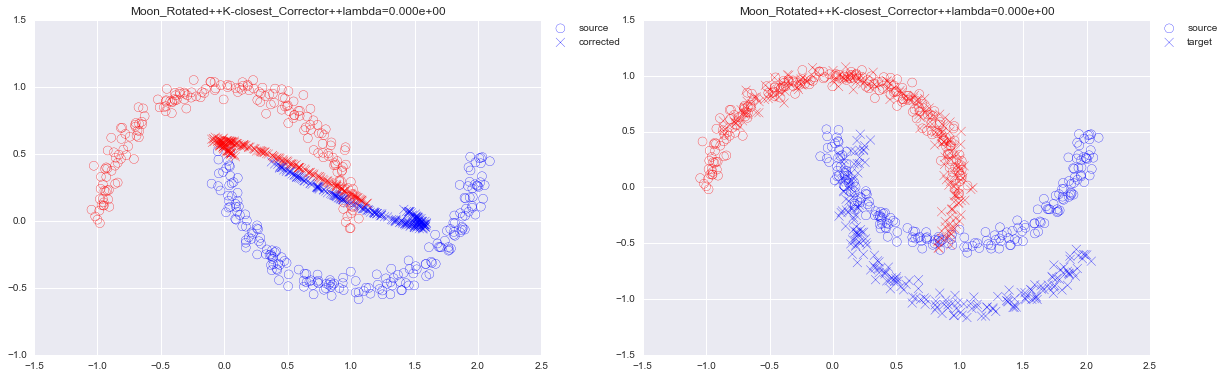
\includegraphics[width=\linewidth]{fig/21-04-2016/exhaustive-pb.png}
\caption{Correction avec les k-plus proches voisins entre les données}
\label{fig:exhaustive-pb}
\end{figure}

Une piste possible pour éviter cet écrasement des données serait de forcer le 
réseaux à ne pas perdre de l'information en lui demandant de reconstruire les
données \emph{Cible} après leurs corrections (figure \ref{fig:de-correcteur}).

\begin{figure}[H] % images
\centering
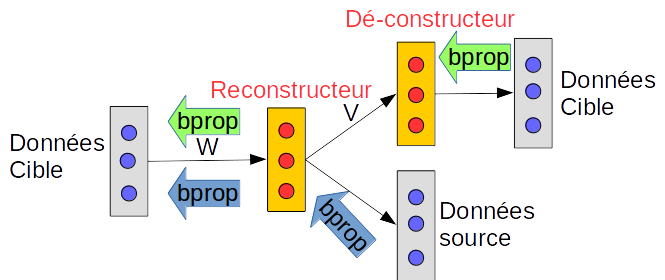
\includegraphics[width=0.45\linewidth]{fig/21-04-2016/Re-De-constructeur.png}
\caption{Correction sous contrainte de dé-correction possible}
\label{fig:de-correcteur}
\end{figure}

Voir même, rêvons un peu, rendre cette partie récurrente (figure \ref{fig:recurrent-de-correcteur}).
\begin{figure}[H] % images
\centering
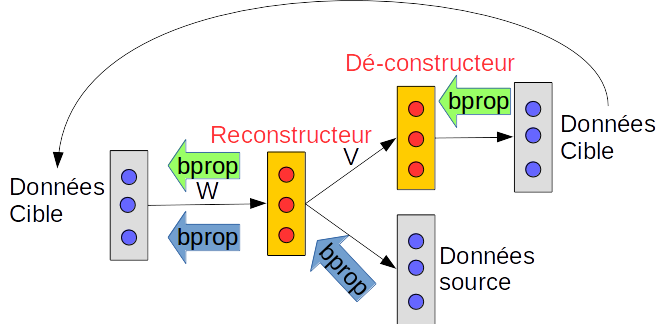
\includegraphics[width=0.45\linewidth]{fig/21-04-2016/Recurrent-correcteur.png}
\caption{Correction sous contrainte de dé-correction possible, version récurrente}
\label{fig:recurrent-de-correcteur}
\end{figure}

Enfin le temps de calcul ne passe pas à l'échelle (complexité $\mathcal O (n^2)$).
Malgré la parallélisation avec GPU, sur MNIST la plupart du temps de calcul 
est alloué aux calculs des distances 2 à 2 (150 sec par époque contre 1.5 sec 
pour le NN).

Cette méthode est aussi trop sensible à l'initialisation. En fait elle 
requiert que l'initialisation résolve le problème.

\experiment{K-moyennes}

Pour palier au problème de l'algo exhaustif on peut construire des clusters. 
Puisque le problème est résolu pour les simples nuages de points, il suffit 
de se ramener à ce problème. On va donc sous-diviser les données \emph{Sources}
et les données \emph{Cible} en petits paquets à l'aide de K-moyennes.

Intérêts:
\begin{enumerate}
	\item Le calcul des distances 2 à 2 reste quadratique mais sur un petit 
	nombre de points. Donc faisable.
	\item On va ainsi capturer les formes des distributions plus complexes (si
	on donne suffisamment de clusters).
\end{enumerate}

\textbf{Notations :} (Les notations de la section précédente n'étaient pas très intuitive)
\begin{description}
\item[$S_i$] les clusters de la distribution \emph{Source} 
	($S_i \subset \mathcal X_S$)
\item[$s_i$] les centres des clusters de la distribution \emph{Source} 
\item[$C_i$] les clusters de la distribution \emph{Cible} 
	($C_i \subset \mathcal X_T (= \phi(\mathcal X_S)$)
\item[$c_j$] les centres des clusters de la distribution \emph{Cible}  
\item[$C_i^\prime$] les clusters de la distribution \emph{Corrigée} 
	($C_i^\prime \subset \mathcal \psi(\mathcal X_T) )$ 
\item[$c_j^\prime$] les centres des clusters de la distribution \emph{Corrigée}
\end{description}

Remarques :

Si $\phi$ ne change pas les distances alors on peut raisonnablement 
espérer (démo ?) qu'il existe une association $c_j = \phi(s_i)$. Cependant il 
est toujours vrai que $c_j^\prime = \psi(c_j)$ par définition.


Maintenant nous allons nous pencher sur les problèmes de cette méthode et 
les solutions possibles.


\subexperiment{Ambiguïté}

Nous utilisons donc 2 K-moyennes, un pour construire $k$ clusters dans la 
distribution \emph{Source} (notés $S_i$) et un pour construire $k$ clusters
dans la distribution \emph{Cible} (noté $C_i$). Ces derniers servent à
obtenir des clusters $C_i^\prime = \psi(C_i)$ en passant les points de $C_i$
dans le \emph{correcteur} (ici un réseau de neurone).

Je pensais ce problème analogue à celui des nuages de points qui fonctionnait
très bien. En fait NON. On ignore quel cluster $C_i$ va avec quel cluster
$S_i$ contrairement aux nuages de points où on connaissait déjà cet alignement !

On arrive donc au premier problème, \textbf{l'ambiguïté}. Le \emph{correcteur}
se retrouve bloqué si il se trompe sur l'alignement de certain cluster.

\begin{figure}[H] % images
\centering
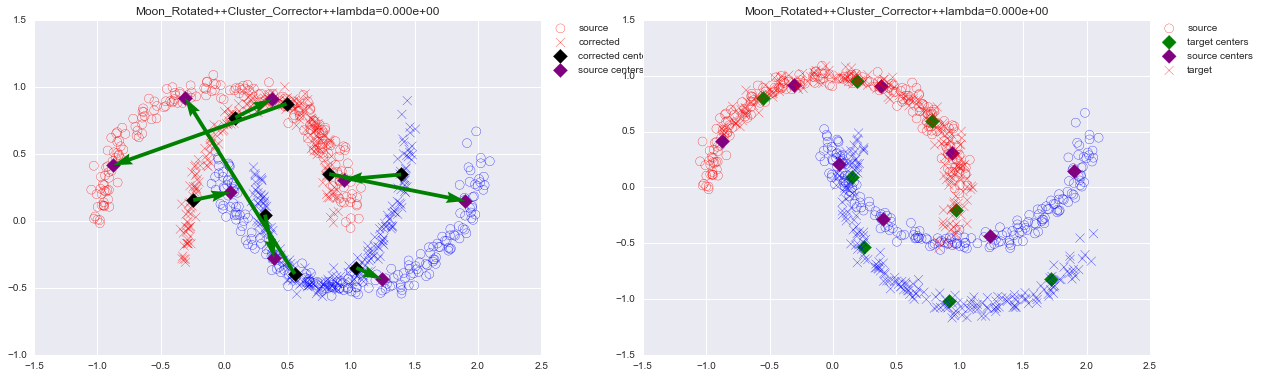
\includegraphics[width=\linewidth]{fig/21-04-2016/stuck_blue-red.png}
\caption{Ambiguïté du choix de l'alignement}
\label{fig:stuck_red_blue}
\end{figure}
On observe sur la figure \ref{fig:stuck_red_blue} que les clusters corrigés 
(en noir) sont alignés (flèches) sur les mauvais clusters sources (en violet).
Ce problème bloque le correcteur dans un état ``tiraillé'' ou ``oscillant''.
On observe une ``oscillation'' (ça vibre quoi) des données corrigées quand 
on regarde chaque époque l'une après l'autre.

Ce problème peut être absorbé par l'utilisation des classes. Ici les deux 
lunes sont ``interchangeables'', une solution à l'alignement pourrait être 
de mettre les bleus sur les rouges et les rouges sur les bleus.
Utiliser les classes (information dont on dispose après tout) peut 
désambiguïser. Enfin presque ! Dans le cas de la figure \ref{fig:stuck_2}
on a une seule erreur (permutation de 2 clusters) qui empêche le correcteur
d'atteindre un résultat parfait.

\begin{figure}[H] % images
\centering
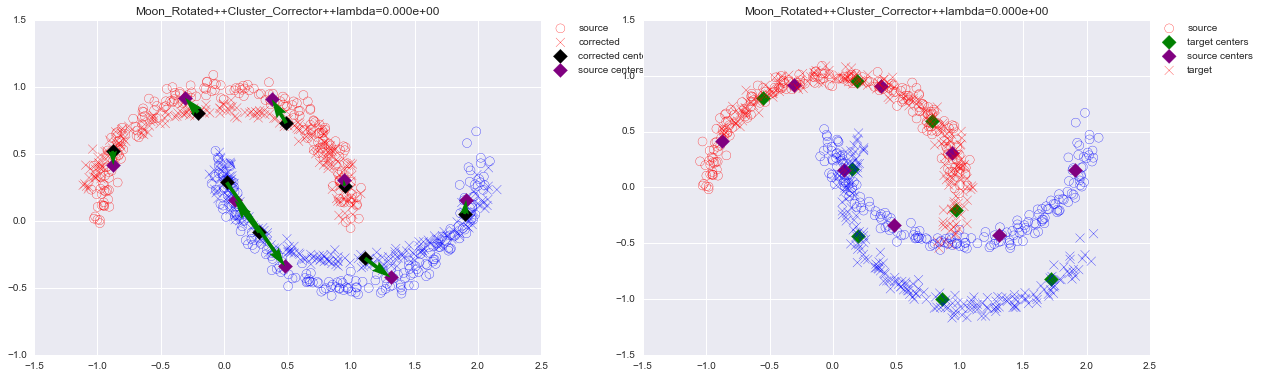
\includegraphics[width=\linewidth]{fig/21-04-2016/Stuck_2.png}
\caption{Ambiguïté du choix de l'alignement}
\label{fig:stuck_2}
\end{figure}


\subexperiment{Initialisation}

Ces derniers résultats sont assez encourageant. Cependant ils ont été obtenus
après moult essais. En effet la méthode est très sensible à l'initialisation.

\textcolor{red}{Erratum} : les expériences de Lundi, 25 avril matin montre que 
l'initialisation ne pose plus vraiment de problème pour le problème des 
demi-lunes. Si on utilise suffisamment de clusters (4) le correcteur réussit 
au bout de quelques époques.
Cependant trop de cluster tue l'efficacité du correcteur (ambiguïté) exemple
figure \ref{fig:stuck_trop}.

\begin{figure}[H] % images
\centering
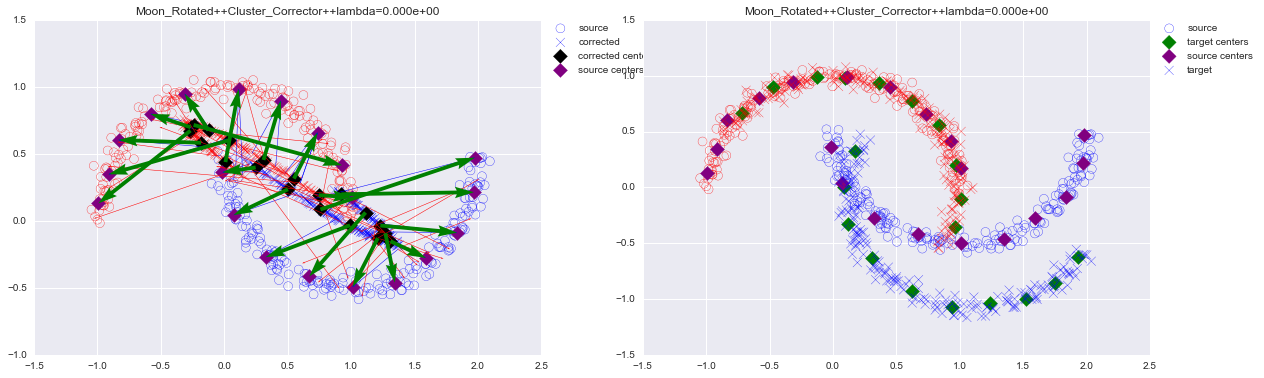
\includegraphics[width=\linewidth]{fig/21-04-2016/Stuck_trop.png}
\caption{Ambiguïté du choix de l'alignement}
\label{fig:stuck_trop}
\end{figure}

Bref. L'initialisation reste probablement un problème clé pour l'entraînement 
du correcteur, une mauvaise initialisation pouvant amener à des cas 
pathologiques.

Solutions : 
\begin{enumerate}
	\item Lancer 50 initialisations et prendre la meilleure, ce qui requiert
une mesure fine de la performance de la correction.
	\item Initialiser proche de l'identité, cela requiert l'hypothèse que 
la solution en est proche. Cela reste une méthode pour utiliser les 
connaissances expertes sur le problème. De plus elle est compatible avec
la précédente.
\end{enumerate}

% TODO : 
\subexperiment{Autres}

Quid du cas où $\phi$ ajoute ou divise des distributions ? Dans ce cas le 
correcteur ne doit pas simplement renvoyer un point sur un autre mais aussi 
discriminer les points importants des parasites. De plus l'hypothèse de $\phi$
conservant les distances ne tient plus.
(faire un exemple avec Clouds)

Créer de nouveaux toys ! Si on avait pas utilisé les Moons j'aurais raté 
pleins de problèmes ! Qui sait ce qu'on rate encore ? De façons générale il 
faut tester les limites de la méthode et trouver des moyens pour diagnostiquer
les cas pathologiques pour appliquer les bonnes corrections.

\begin{figure}[H] % images
\centering
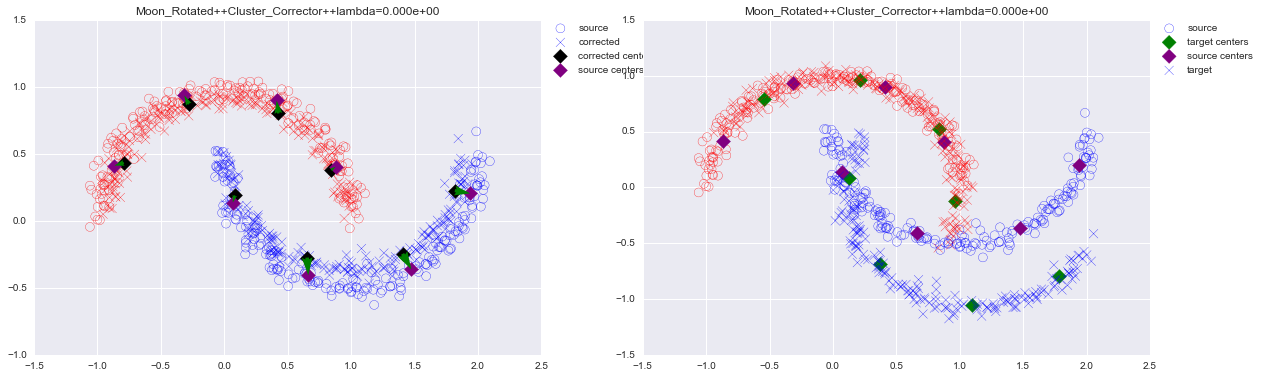
\includegraphics[width=\linewidth]{fig/21-04-2016/good_init.png}
\caption{Quand ça marche}
\label{fig:good_init}
\end{figure}


\subexperiment{Résumé des Pistes}
\begin{enumerate}
	\item Mesure plus fine des performances du correcteur. KL, comparaison des
	histogrammes des clusters, de leur variance à inclure dans la distance
	\item Initialisation multiple + choix de la meilleure.
	\item Initialiser selon les connaissances expertes (à l'identité par exemple)
	\item Créer de nouveau Toys pour tester la robustesse de la méthode face 
	à divers types de transformation.
	\item Rendre le choix de l'alignement des clusters moins déterministe 
	(pour éviter figure \ref{fig:stuck_2})
\end{enumerate}


%----------------------------------------------------------------------------------------
